\section*{Antecedentes}
\markboth{\MakeUppercase{Antecedentes}}{}
\addcontentsline{toc}{section}{Antecedentes}

El software desarrollado en este trabajo toma como base al emokit\cite{emokit} el cu�l forma parte de OpenYou\cite{emokit}. El Emokit lee, descifra e interpreta la informaci�n enviada por el Emotiv EPOC, el cual es un dispositivo ``Interfaz Cerebro-M�quina'' (BCI), tales como nivel de bater�a de la diadema, intensidad de la se�al, y las 14 lecturas realizadas por la diadema; este software actualmente solo imprime a nivel terminal dichos datos.
\subsection*{BCI}
\markboth{\MakeUppercase{BCI}}{}
\addcontentsline{toc}{subsection}{BCI}

Una ``Interfaz Cerebro-M�quina''\cite{2012bci} (BCI) es un medio de comunicaci�n directo entre el cerebro y un dispositivo externo. Los BCI est�n normalmente dirigidos a asistir, aumentar y reparar la habilidad cognitiva y las funciones sensoriomotoras.
\\ Las inventigaciones con los BCI comenzaron en 1970 en la Universidad de Los �ngeles California(UCLA) bajo el subsidio de Fundaci�n Nacional de Ciencia contratados por la Agencia de Proyectos de Investigaci�n Avanzados de Defensa (DARPA). La publicaci�n hecha despu�s de la investigaci�n marc� la primera aparici�n de la expresi�n ``Interfaz Cerebro-M�quina'' en la literatura cient�fica.


Existen diferentes formas de clasificar a los BCI.
\paragraph*{Por el uso de t�cnicas invasivas}
\begin{itemize}
\item BCI invasivos.
%\item BCI semi invasivos.
\item BCI no invasivos.
\end{itemize}

\paragraph*{Por el uso de estimulaci�n}
\begin{itemize}
\item End�genos
\item Ex�genos
\end{itemize}

\paragraph*{Por las caracter�sticas EEG}
\begin{itemize}
\item Sistemas BCI basados en potenciales corticales lentos
\item Sistemas BCI basados en ritmos de actividad cerebral
\item Sistemas BCI basados en potenciales evocados
\end{itemize}

\subsubsection*{BCI Invasivos}
\markboth{\MakeUppercase{BCI Invasivos}}{}
\addcontentsline{toc}{subsubsection}{BCI Invasivos}

Los dispositivos BCI invasivos son implantados directamente en el cerebro y tienen la m�s alta calidad de se�ales de los BCI. Estos dispositivos son usados para recuperar funciones de personas con par�lisis. Los BCI invasivos son usados tambi�n para recuperar la vista conectando el cerebro a c�maras externas y para restaurar el uso de extremidades usando brazos y piernas rob�ticos controlados por el cerebro. Como todos los dispositivos que se encuentran instalados en la materia gris del cerebro este tipo de BI produce una calidad de se�ales muy alta pero son propensos a causar cicatrices en el tejido cerebral causando que las se�ales comiencen a volverse d�biles o incluso la p�rdida de las reacciones del cuerpo por contener un objeto desconocido en el cerebro\cite{invasiveBCI1}. \\
En las ciencias de la visi�n los implantes en el cerebro han sido usados para tratar la ceguera no cong�nita\footnote{Una enfermedad cong�nita es aquella que se manifiesta desde el nacimiento, ya sea por un trastorno ocurrido durante el desarrollo embrionario, durante el parto o como consecuencia de un defecto hereditario}. William Dobell es uno de los primeros cient�ficos que vienen trabajando con una interfaz cerebro para restaurar la vista como una investigaci�n privada. El implant� su primer prototipo en Jerry, un hombre que qued� ciego en su adultez en 1978. �l insert� un BCI de 68 electrodos en la corteza visual de Jerry y logr� producir la sensaci�n  de ver una luz. En 2012 el experimento fu� realizado en Jens Neumann donde Dobell utiliz� un implante m�s sofisticado que permiti� un mejor mapeo. Investigadores de la Universidad de Emory en Atlanta, dirigidos por Philip Kennedy y Roy Bakay fueron los primeros en instalar un implante en el cerebro de un ser humano que produce se�ales de alta calidad suficientes para estimular el movimiento\cite{invasiveBCI1}. \\
Thomas Navin Lal et al. en su art�culo \cite{invasiveBCI2} desarrollaron un BCI llamado Thought Translation Device (TTD) es cual usan para ayudar a comunicarse a pacientes con par�lisis los cu�les han perdido sus funciones cognitivas. Para poder usar el TTD los pacientes debieron aprender a regular a voluntad su Slow Cortical Potentials (SCP)\footnote{Se llaman SCP (o potenciales corticales lentos en espa�ol) a los cambios relacionados con los eventos de corriente continua lenta obtenidas con los EEG provenientes de los grandes conjuntos de c�lulas en la capa cortical superior\cite{SCP:Online}.}. El sistema entonces permite a su usuario escribir textos en la pantalla de una computadora o navegar en internet. El sistema sin embargo cuenta con dos desventajas: no todos los pacientes logran controlar su SCP adem�s la intensidad de la se�al es un poco baja y a un usuario bien entrenado requiere aproximadamente 30 segundos para escribir un caracter. % insertar imagen del articulo
\\
Niels Birbaumer publica en su art�culo\cite{birbaumer2006breaking} el resultado de su investigaci�n donde analiza a los BCI invasivos y no invasivos desde la perspectiva de su utilidad cl�nica para la comunicaci�n y reparaci�n de habilidades motoras en personas con par�lisis. En su investigaci�n encontr� publicaciones de distintos casos de Esclerosis Lateral Amiotr�fica (ELA)\footnote{ELA es una enfermedad degenerativa de tipo neuromuscular. Se origina cuando unas c�lulas del sistema nervioso llamadas motoneuronas disminuyen gradualmente su funcionamiento y mueren, provocando una par�lisis muscular progresiva de pron�stico mortal} en diferentes estados. A los pacientes se les implanto un microelectrodo de vidrio cortical lleno de un factor de crecimiento neurotr�fico. Con dicho implante los pacientes lograron comunicarse apagando y encendiendo un flash-ion para decir ``si'' y ``no'' sin embargo el autor citado concluye que es complicado realizar un juicio a cerca de los BCI invasivos debido a las complicaciones m�dicas que puede conllevar. En esta misma publicacion se menciona una conferencia sobre BCI realizada en Rennselearville, Nueva York en 2005 donde a los m�s de 100 cient�ficos que asisteron se les pregunt� su opinion sobre el futuro de los BCI. La mayor�a opin� que los BCI no invsivos ser�a el desarrollo m�s prometedor de la siguiente d�cada.

\begin{figure}[bp!]
\centering
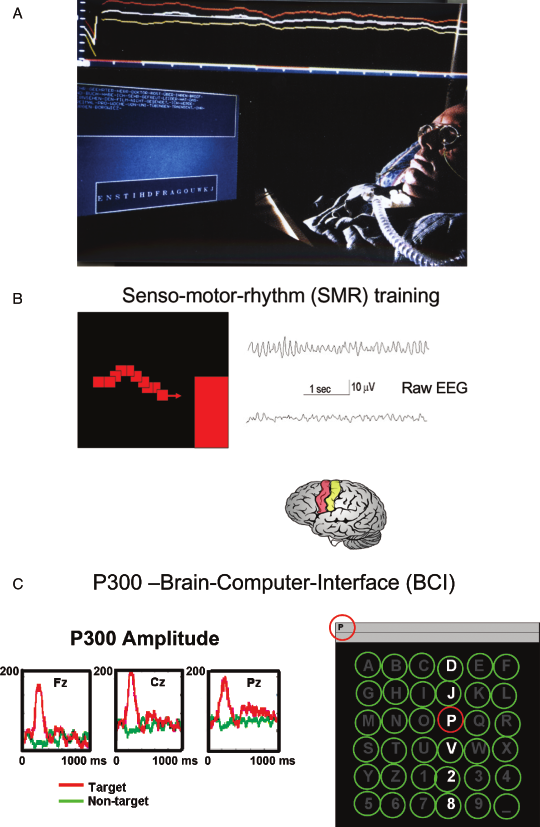
\includegraphics[width=.6\textwidth]{img/bci-invasivo.png}
%
\includegraphics[scale=1,bb=0 0 30 30]{img/bci1.jpg}
\caption{Tres tipos de BCI. A: Pacientes usando su Slow Cortical Potentials. Los pacientes seleccionan una letra de las mostradas en la parte baja de la pantalla, la letra seleccionada aparece en la parte de arriba de la pantalla. B: SMR-BCI. Oscilaciones SMR de la corteza sensoriomotora durante la inhibici�n del movimiento y las im�genes o ejecuci�n de movimiento (EEG rastro abajo). En la parte izquierda de la imagen es la pantalla de retroalimentaci�n con el objetivo de destino en el lado derecho de la pantalla que indica el aumento requerido SMR (objetivo en la parte inferior) o disminuir SMR (objetivo en la parte superior). El cursor refleja el SMR actual se representa en movimiento rojo de la parte derecha de la pantalla hacia la meta de destino. C: P300-BCI: Filas y columnas de letras son resaltadas en suseciones r�pidas, siempre que la letra pensada se encuentre en la cadena iluminada un P300 aparece en el EEG. Tomada de \cite{birbaumer2006breaking}} 
% \footnote{La onda P300 es un potencial evocado que puede ser registrado mediante electroencefalograf�a como una deflexi�n positiva de voltaje con una latencia de unos 300ms en el EEG}
\label{fig:bci-invasivos}
\end{figure}

%\subsubsection*{BCI semi Invasivos}
\markboth{\MakeUppercase{BCI semi Invasivos}}{}
\addcontentsline{toc}{subsubsection}{BCI semi Invasivos}

Son implantados dentro del cr�neo pero sin tocar la corteza cerebral. Producen una mejor se�al que los BCI no invasivos y tienen menor riesgo de causar da�os al cerebo que los BCI invasivos.
\subsubsection*{BCI no Invasivos}
\markboth{\MakeUppercase{BCI no Invasivos}}{}
\addcontentsline{toc}{subsubsection}{BCI no Invasivos}

Los implantes no invasivos son colocados en el cuero cabelludo. Los BCI no invasivos producen se�ales d�biles porque el cr�neo amortigua las se�ales, dispersando las ondas electromagn�ticas creadas por las neuronas.
\\
Javier Danilo et al. describen es su trabajo de titulaci�n\cite{asimbaya2014diseno} el dise�o e implementaci�n de un prototipo de BCI para manipular una pinza rob�tica. A trav�s de electrodos colocados en el cuero cabelludo de una persona y utilizando los principios de la electroencefalograf�a (EEG) obtienen se�ales el�ctricas peque�as las cuales someten a etapas de amplificaci�n y filtrado de ruido. Para la adquisici�n de las se�ales utilizan la plataforma Arduino, y haciendo uso de la comunicaci�n serial con el software MATLAB para la visualizaci�n en la computadora de las se�ales obtenidas. Posteriormente se identificar�n los pulsos el�ctricos que son generados por un est�mulo visual y que ser�n los que determinen la activaci�n de un mecanismo. Este mecanismo manipular� a un dispositivo a distancia
que en este caso ser� una pinza rob�tica.
\begin{figure}[htb]
\centering
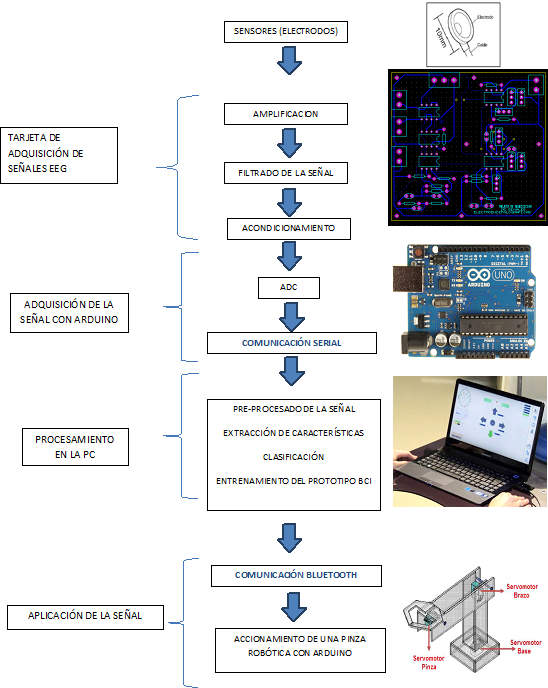
\includegraphics[width=.5\textwidth]{img/bci-brazo-robotico.png} \label{fig:bci-brazo-robotico}
\caption{La imagen describe el dise�o del prototipo de Danilo\cite{asimbaya2014diseno} }
\end{figure}
\\
Miguel �ngel L�pez en su tesis doctoral \cite{gordo2009interfaz} dentro de la clasificaci�n de los BCI describe a los BCI no Invasivos como aquellos m�todos que no suponen riesgo alguno para el paciente. Entre los BCI no invasivos se encuentran los EEG, MEG, fMRI y NIRS destacando a los EEG como la alternativa m�s importante, sencilla y econ�mica de la actualidad. La EEG se basa en el principio de que las corrientes de naturaleza i�nica, presentes en la corteza cerebral, producto de la actividad poblaciones de neuronas pueden ser registradas para su an�lisis mediante el uso de electrodos superficiales extracraneales. Existen tambi�n distintas t�cnicas para la fijaci�n de los electrodos. Una t�cnica consiste en el uso de un gorro con una serie de agujeros donde ajustar mediante rosca los electrodos, esta t�cnica tiene el inconveniente de tener que ajustar uno a uno cada electrodo, junto con un gel electrolito. Una versi�n mejorada, Electrocap, dispone de los electrodos ya integrados en el gorro y de un sistema c�modo de aplicaci�n del gel. Existen tambi�n redes de sensores, como el SensorNet de EGI. Este �ltimo consiste en una red el�stica que se ajusta a la cabeza de cada sujeto con un n�mero muy elevado de sensores (hasta 250).
\begin{figure}[htb]
\centering
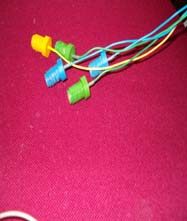
\includegraphics[scale=.6]{img/colocacion-bci1.png} \label{fig:colocacion-bci1}

\includegraphics[scale=1.35]{img/colocacion-bci2.png} \label{fig:colocacion-bci2}
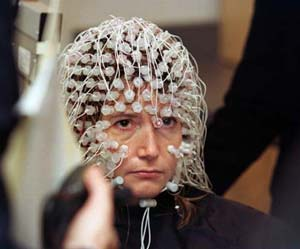
\includegraphics[scale=.5]{img/colocacion-bci3.png} \label{fig:colocacion-bci3}
\caption{Sistemas de sujeci�n de electronos EEG.De izquierda a derecha. Electrodos usados en un gorro EEG con agujeros y rosca, el Electrocap y el SensorNet de EGI. Tomadas de \cite{gordo2009interfaz}}
\end{figure}
\\
El uso de redes o sensores resultan �iles para aplicaciones m�dicas sin embargo esas interfaces resultan poco atractivas en el �mbito del entretenimiento. Empresas como NeuroSky y Emotiv han desarrollado cascos para el sector del entretenimiento que ofrecen un sistema r�pido, c�modo y portatil.
\begin{figure}[htb]
\centering
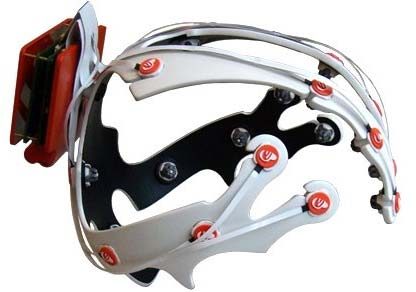
\includegraphics[scale=.5]{img/emotiv.png} 

\includegraphics[scale=.9]{img/neurosky.png} 
\caption{Sistemas comerciales BCI: Emotiv a la izquierda y NeuroSky a la derecha. Tomado de \cite{gordo2009interfaz}} \label{fig:bci-comerciales} 
\end{figure}

\begin{figure}[htb]
\centering
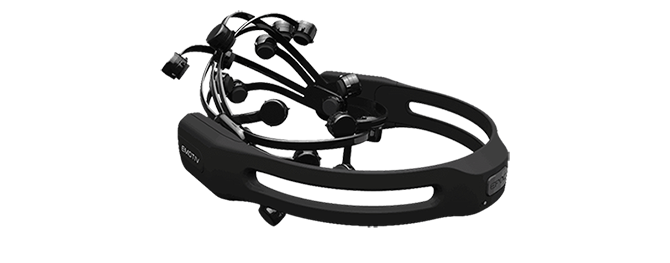
\includegraphics[width=0.8\textwidth]{img/epoc.png}
%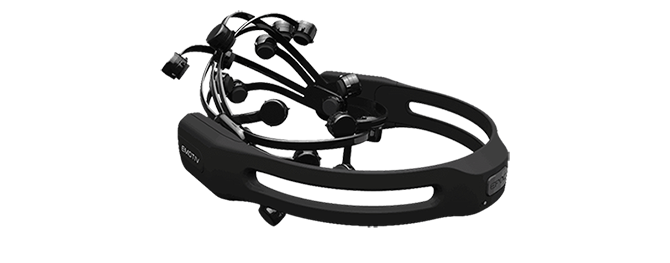
\includegraphics[scale=1,bb=0 0 30 30]{img/epoc.png}
\caption{BCI no invasivo\cite{emotiv:Online}} \label{fig:bci2}
\end{figure}
%Queda pendiente otra clasificacion econtrada en gordo2009interfaz pag78

El Emotiv Epoc es BCI que fue creado con el prop�sito de ser un perif�rico para juegos en Windows, OS X y Linux\cite{Emotiv:Wiki:Online}, cuenta con 14 electrodos y funciona como dispositivo de entrada. En 2011 Kirill Stytsenko, et al.\cite{stytsenko2011evaluation} realizaron un an�lisis del Emotiv EPOC para la CogSci Conference. Emotiv EPOC es un BCI de bajo costo basado en la tecnolog�a EEG. Cuenta con 14 electrodos montados en una diadema inal�mbrica que se coloca sin esfuerzo y se conecta a la computadora. Originalmente fue creada para los juegos de computadora pero la ``research edition'' permite el acceso a los datos para su an�lisis lo que abre nuevas posibilidades a la ciencia para realizar nuevos experimentos o integrarlo a los ya existentes. En dicho estudio se someten a diferentes pruebas al Emotiv EPOC y al G-TEC\cite{G-TEC:Online}. Al compararlos se obtiene que la informaci�n en general es igual, pero la se�al es m�s clara e intensa en el G-TEC. Uno de los desaf�os encontrados es la creaci�n de software de grabaci�n para ambos dispositivos.
\\ Job Ram�n de la O Ch�vez en su tesis Interfaz Cerebro - Computadora para el Control de un Cursor Basado en Ondas\cite{intcerebro} plantea una interfaz que permita la comunicaci�n entre el usuario y la computadora, haciendo uso de sus ondas cerebrales, para el control de un cursor en pantalla mediante comandos obtenidos de las lecturas de un amplificador de ondas cerebrales.
\\ En EPOC-alypse Mind Controlled Car\cite{seniorepoc} plantean la construcci�n de de un carro de control remoto que es controlado por la mente usando el Emotiv EPOC. El proyecto fue desarrollado utilizando el SDK oficial del Emotiv EPOC.
\\ Asim Raza en SSVEP based EEG Interface for Google Street View Navigation\cite{raza2012ssvep} analiza los sistemas BCI y su aplicaci�n en el mundo real. Tambi�n desarrolla un prototipo interactivo que pueda ser controlado en un ambiente controlado para demostrar el funcionamiento de los sistemas BCI. Para el desarrollo decidi� utilizar el software libre OpenViBE para la adquisici�n y procesamiento de las se�ales.
\\ En ROS: an open-source Robot Operating System\cite{2009ros} se explica el uso de la plataforma ROS para el desarrollo de aplicaciones de rob�tica y resumen los objetivos filos�ficos de ROS en:
\begin{itemize}
\item Per-to-per
\item Basado en herramientas
\item Multilenguaje
\item Ligero
\item Gratuito y de C�digo Abierto
\end{itemize}
%ROS provee una capa de comunicaci�n estructura basada en Peer-to-peer, basado en herramientas, adem�s es multilenguaje, ligero, gratuito y de c�digo abierto.
En Things that twitter: social networks and the internet of things\cite{kranz2010things} utilizan ROS aplicado en las redes sociales. ROS permite intercambiar informaci�n por medio de servicios con mensaje de request y response definidos. La informaci�n es intercambiada por una arquitectura publish/suscribe donde los procesos permiten que sus datos est�n disponibles para que otros procesos puedan utilizarlos.

% Trabajos sobre cda tipo de BCI, enfatizar no invasivo.
% LIrbos, publicaciones etc que hablen sobre ellos.
% aplicacion en los videojuegos
% Avance de las compa�ias en el tema de los BCI
% Quienes han investigado sobre BCI
% Paises avanzados en el campo
% Campos con los que se relaciona